\chapter{Methodology}
\label{chap:methodology}
Here the methodology used to develop and test the software will be detailed. This will include the tools used, the development process and the testing process. Using the appropriate methodology is key to the success of a project and will ensure that the required features are implemented within the required timescale.
\section{Development}
\label{methodology:development}
Whilst there are many software development approaches, Kanban was chosen as the best methodology because only one person will be working on the development of the software, not a team of developers. Kanban is a simple and effective way to manage a single person’s workload and is a good fit for this project. A solution such as Trello, \cite{trello}, can be utilised as it is free for small teams and is quick and easy to use. The Trello board that will be used for development is shown in figure \ref{fig:kanban-board}.

\begin{figure}[H]
    \centering
    
\includegraphics[scale=0.2]{images/trello-board.png}
    \caption{Trello Kanban board used to manage the development process}
    \label{fig:kanban-board}
\end{figure}

The project requirements will be broken down into smaller tasks, and each task will be added to the Trello board. The tasks will be added to the “To Do” column and then moved to the “Doing" column when the task is being worked on. Once the task is complete, it will be moved to the “Done” column. This will allow the project to be broken down into smaller tasks and will allow the project to be managed effectively. The tasks will be added to the board in the order that they are required to be completed, and will be worked on in that order. This will ensure that the project is completed in the correct order and will ensure that the project is completed in the required timescale.
There are also 2 other lists, namely "Bugs" and "Resolved Bugs" which will allow for the ease of tracking bugs and ensuring that they are resolved during the development cycle.

\section{Time Management}
\label{methodology:time-management}
To ensure that the project keeps to time, a Gantt chart is to be used which will outline the key milestones of the project and when they should be met. To generate this chart, \cite{teamgantt}, was used as it has a free tier and meets all of the requirements for this project. Figure \ref{fig:gantt-chart} shows the Gantt chart for the project.
\begin{figure}[H]
    \centering
    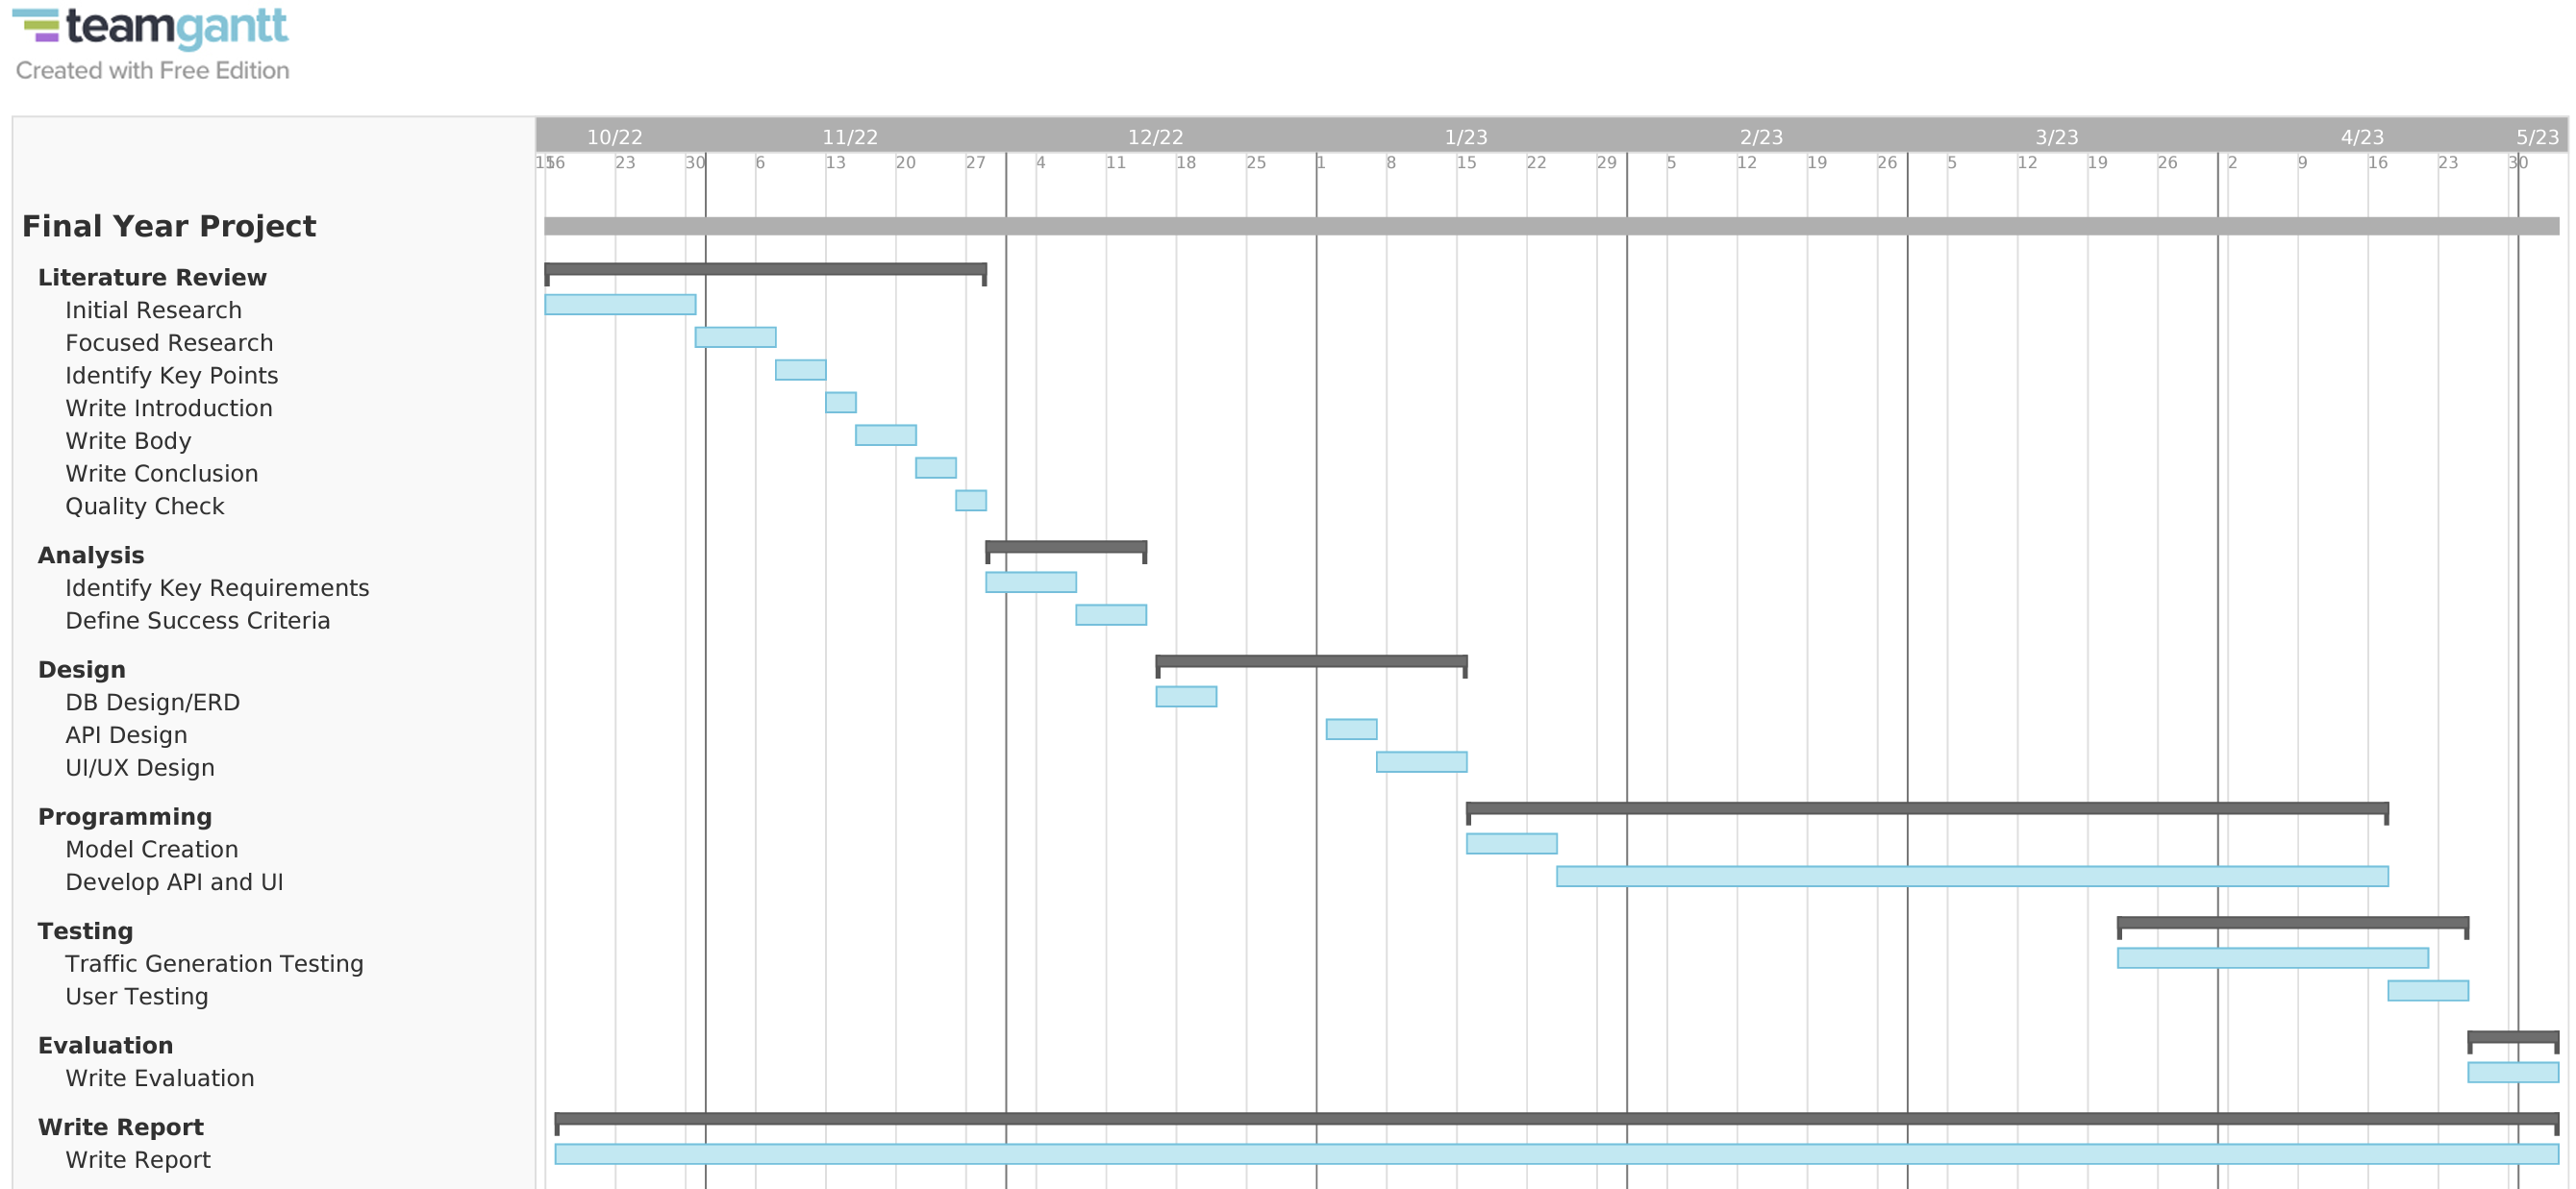
\includegraphics[scale=0.2]{images/gantt-chart.png}
    \caption{Gantt chart used to outline the key project milestones}
    \label{fig:gantt-chart}
\end{figure}
As the project will follow the Kanban development methodology, some stages overlap and will occur simultaneously. This is because testing will be critical to influencing the development process and ensuring that features work correctly as they are developed. The tight timescale of this project also means that tight features be tested as they are written to prevent issues later in the project.
\section{Project Management}
\label{methodology:project-management}
To ensure secure storage, accessibility and history of code as it is written, Git will be used to manage the project. Git is a version control system that allows for the tracking of changes to code and the ability to revert to previous versions of the code. GitHub will be used to host the code and will allow for the code to be accessed from anywhere, GitHub also has a free tier which will be used for this project. The GitHub repository for this project can be found at \url{https://github.com/mattg66/fyp}.